% figure1_pair_radial.tex — (a) PiKV-style block diagram (top) + (b) radial
% RepairKV hub (bottom). RepairKV pill sits at the visual centre with three
% internal sub-pills (score / top-K / promote). Host pool sits on the left,
% GPU active sits on the right; signal s enters from above. Three short
% straight arrows connect Host -> RepairKV -> GPU and signal -> RepairKV.
%
% Style harmonised with figure1_pikv.tex: sharp-cornered rectangles, 0.5pt
% black outline, white fill, single pale-blue accent on GPU active, dashed
% orange "Host" group, no curves.
% Shared preamble for standalone Figure 1 variants.
\documentclass[border=8pt,tikz]{standalone}
\usepackage{amsmath}
\usepackage{amssymb}
\usepackage{tikz}
\usetikzlibrary{arrows.meta,positioning,calc,fit,shapes.geometric,backgrounds}
\usepackage{xcolor}
\usepackage[T1]{fontenc}
\usepackage{mathptmx}
\newcommand{\repairkv}{\textsc{RepairKV}}
\newcommand{\bbase}{\ensuremath{B_{\mathrm{base}}}}
\newcommand{\bmatch}{\ensuremath{B_{\mathrm{match}}}}

\begin{document}
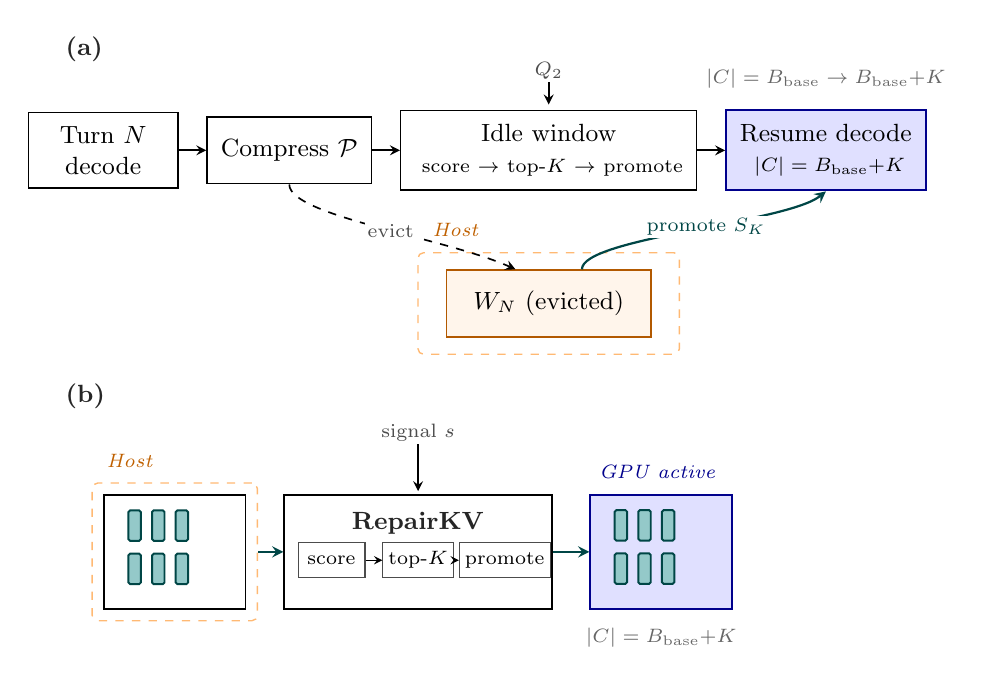
\begin{tikzpicture}[
  >=latex, line width=0.4pt,
  font=\small,
  % --- (a) pikv styles (kept identical to figure1_pikv.tex) ---
  box/.style={draw=black, fill=white, line width=0.5pt,
              inner sep=5pt, align=center, minimum height=0.85cm},
  active/.style={box, fill=blue!12, draw=blue!55!black, line width=0.7pt},
  store/.style={box, fill=orange!8, draw=orange!70!black},
  arr/.style={->, line width=0.6pt, draw=black, >=stealth},
  promarr/.style={->, line width=0.8pt, draw=teal!55!black, >=stealth},
  arrlabel/.style={font=\scriptsize, text=black!70, fill=white, inner sep=1pt},
  groupbox/.style={draw=orange!55, dashed, line width=0.5pt, rounded corners=2pt},
  grouplabel/.style={font=\scriptsize\itshape, text=orange!75!black},
  panellabel/.style={font=\bfseries\small, text=black!85},
  bodysmall/.style={font=\scriptsize, text=black!75},
  % --- (b) radial hub styles ---
  hubpill/.style={draw=black, fill=white, line width=0.6pt,
                  inner sep=6pt, align=center, minimum height=1.45cm,
                  minimum width=3.4cm},
  subpill/.style={draw=black!70, fill=white, line width=0.4pt,
                  inner sep=2pt, align=center, minimum height=0.45cm,
                  minimum width=0.85cm, font=\scriptsize},
  hostpool/.style={draw=black, fill=white, line width=0.5pt,
                   inner sep=5pt, align=center, minimum height=1.45cm,
                   minimum width=1.8cm},
  gpupool/.style={hostpool, fill=blue!12, draw=blue!55!black, line width=0.7pt},
  chip/.style={rounded corners=0.6pt, minimum width=4.5pt, minimum height=11pt,
               inner sep=0pt, line width=0.5pt},
  tealchip/.style={chip, draw=teal!55!black, fill=teal!42, line width=0.7pt}
]
  % =================================================================
  % Panel (a) — PiKV block diagram (top); identical layout to figure1_pikv
  % =================================================================
  \node[panellabel, anchor=south west] at (0, 4.4) {(a)};

  \node[box, minimum width=1.9cm] (dN) at (0.6, 3.4) {Turn $N$\\decode};
  \node[box, minimum width=1.7cm, right=10pt of dN]   (cmp)  {Compress~$\mathcal{P}$};
  \node[box, minimum width=2.7cm, right=10pt of cmp]  (idle)
       {Idle window\\{\scriptsize{} score~$\to$~top-$K$~$\to$~promote}};
  \node[active, minimum width=2.1cm, right=10pt of idle] (resume)
       {Resume decode\\{\scriptsize{} $|C|=\bbase{+}K$}};

  \draw[arr] (dN) -- (cmp);
  \draw[arr] (cmp) -- (idle);
  \draw[arr] (idle) -- (resume);

  \draw[arr] ([yshift=10pt]idle.north) -- ([yshift=2pt]idle.north);
  \node[arrlabel, anchor=south] at ([yshift=10pt]idle.north) {$Q_2$};

  \node[store, minimum width=2.6cm, below=1.0cm of idle] (wn) {$W_N$ (evicted)};
  \node[groupbox, fit=(wn), inner xsep=10pt, inner ysep=6pt] (hgroup) {};
  \node[grouplabel, anchor=south west]
       at ([xshift=2pt, yshift=2pt]hgroup.north west) {Host};

  \draw[arr, dashed]
       (cmp.south) .. controls ([yshift=-0.4cm]cmp.south)
                              and ([yshift=0.4cm]wn.north west) ..
       ([xshift=-12pt]wn.north)
       node[arrlabel, pos=0.55] {evict};

  \draw[promarr]
       ([xshift=12pt]wn.north) .. controls ([xshift=12pt, yshift=0.4cm]wn.north)
                                          and ([xshift=-0.5cm, yshift=-0.4cm]resume.south) ..
       (resume.south)
       node[arrlabel, text=teal!55!black, pos=0.55] {promote~$S_K$};

  \node[bodysmall, text=black!60, anchor=south]
       at ([yshift=4pt]resume.north) {$|C|=\bbase \to \bbase{+}K$};

  % =================================================================
  % Panel (b) — Radial RepairKV hub
  %   Horizontal extent must match (a): x in [0.6, 8.6] (=8 cm).
  %   Layout: Host (left) | RepairKV pill (centre) | GPU active (right).
  %   Signal s enters from above into RepairKV.north.
  % =================================================================
  \node[panellabel, anchor=south west] at (0, 0.0) {(b)};

  % Centre: RepairKV pill at x=4.6 (midpoint of 0.6..8.6), y=-1.7.
  \node[hubpill] (hub) at (4.6, -1.7) {};

  % Title at top of pill
  \node[font=\small\bfseries, text=black!85, anchor=north]
       at ([yshift=-3pt]hub.north) {\repairkv};

  % Three internal sub-pills (score / top-K / promote)
  \node[subpill] (sub1) at ([xshift=-1.1cm, yshift=-3pt]hub.center) {score};
  \node[subpill] (sub2) at ([yshift=-3pt]hub.center)               {top-$K$};
  \node[subpill] (sub3) at ([xshift= 1.1cm, yshift=-3pt]hub.center) {promote};

  % Tiny connecting arrows between sub-pills
  \draw[arr, line width=0.35pt] (sub1.east) -- (sub2.west);
  \draw[arr, line width=0.35pt] (sub2.east) -- (sub3.west);

  % Left: Host pool, anchored so its left edge sits at x=0.6
  \node[hostpool, anchor=west] (host) at (0.6, -1.7) {};
  % Host chips: 6 teal candidates in 2 rows (concrete K-row visualisation)
  \foreach \i in {1,...,3}{
    \pgfmathsetmacro{\xc}{0.30*\i + 0.10}
    \node[tealchip] at ([xshift=\xc cm, yshift=-0.40cm]host.north west) {};
    \node[tealchip] at ([xshift=\xc cm, yshift=-0.95cm]host.north west) {};
  }
  % Host group dashed frame + label
  \node[groupbox, fit=(host), inner xsep=4pt, inner ysep=4pt] (hostg) {};
  \node[grouplabel, anchor=south west]
       at ([xshift=2pt, yshift=2pt]hostg.north west) {Host};

  % Right: GPU active pool, anchored so its right edge sits at x=8.6
  \node[gpupool, anchor=east] (gpu) at (8.6, -1.7) {};
  % GPU chips: 6 teal slots, mirroring host layout (the K rows that landed)
  \foreach \i in {1,...,3}{
    \pgfmathsetmacro{\xc}{0.30*\i + 0.10}
    \node[tealchip] at ([xshift=\xc cm, yshift=-0.40cm]gpu.north west) {};
    \node[tealchip] at ([xshift=\xc cm, yshift=-0.95cm]gpu.north west) {};
  }
  % GPU label (italic, pale blue), placed outside the pool to mirror "Host"
  \node[font=\scriptsize\itshape, text=blue!55!black, anchor=south west]
       at ([xshift=0pt, yshift=2pt]gpu.north west) {GPU active};

  % --- Three short straight arrows ---
  % (1) Host -> RepairKV (left-to-right). Start from the dashed group's east
  %     edge so the arrow is visibly outside the host frame.
  \draw[promarr] (hostg.east) -- (hub.west);
  % (3) RepairKV -> GPU (left-to-right, the K teal chips landing)
  \draw[promarr] (hub.east) -- (gpu.west);

  % (2) Signal s entering from above
  \draw[arr] ([yshift=18pt]hub.north) -- ([yshift=1pt]hub.north);
  \node[arrlabel, anchor=south] at ([yshift=18pt]hub.north) {signal $s$};

  % |C| growth indicator pinned just below GPU pool
  \node[bodysmall, text=black!60, anchor=north]
       at ([yshift=-3pt]gpu.south) {$|C|=\bbase{+}K$};
\end{tikzpicture}
\end{document}
